\documentclass[10pt]{beamer}
\usepackage[utf8]{inputenc}

\usepackage{graphicx}
\usepackage{outlines}
\usepackage[absolute,overlay]{textpos}
\usepackage{hyperref}
\hypersetup{
    colorlinks=true,
    linkcolor=blue,
    filecolor=magenta,      
    urlcolor=cyan,
    pdftitle={Overleaf Example},
    pdfpagemode=FullScreen,
    }
    
\urlstyle{same}

\mode<presentation> {
\usetheme{boxes} % When headline is wanted use Dresden theme instead
\usecolortheme{seagull}
%\logo{
\includegraphics[height=1.5cm]{ku_logo_dk}}
% \setbeamertemplate{footline}[frame number]
\setbeamertemplate{footline}{
  \hspace{1em}
  \hfill
  \insertframenumber/\inserttotalframenumber
  \vspace{1em}
  \hspace{1em}
  
\includegraphics[height=2cm]{ku_logo_dk}
  \hspace{1em}
}
\setbeamertemplate{navigation symbols}{}
\setbeamertemplate{itemize items}[square]
}


%----------------------------------------------------------------------------------------
%	TITLE PAGE
%----------------------------------------------------------------------------------------

\title[Kickstart-kursus] % bottom of every slide
  {Intro Kickstart-kursus i programmering 2023: 1} % title page

\author{\footnotesize{Daniel Spikol, The Team, \& Martin Dybdal}\\
          \footnotesize{\texttt{ds@di.ku.dk}}}

\institute {
DIKU \\ Københavns Universitet
}

\date[14. august 2023]{14.august 2023}

\begin{document}
\begin{frame}[plain]
\titlepage
\end{frame}

%%------------------------%%
%% START %%
\section{Introduction}
\begin{frame}
   \frametitle{Hello World!}
   	 
\includegraphics[height=8cm]{images/week33_image}
\end{frame}

%%------------------------%%

\begin{frame}
 \frametitle{Who are your Instructors}
   \begin{itemize}
   \item Daniel
   \item Anders
   \item Casper
   \item Christian
   \item Jepper
   \item Laufey
   \item Nanna
   \item Nicolaj
   \item Sofie
\end{itemize}
     \hspace{8 em}
%\begin{minipage}{0.4\linewidth} 
      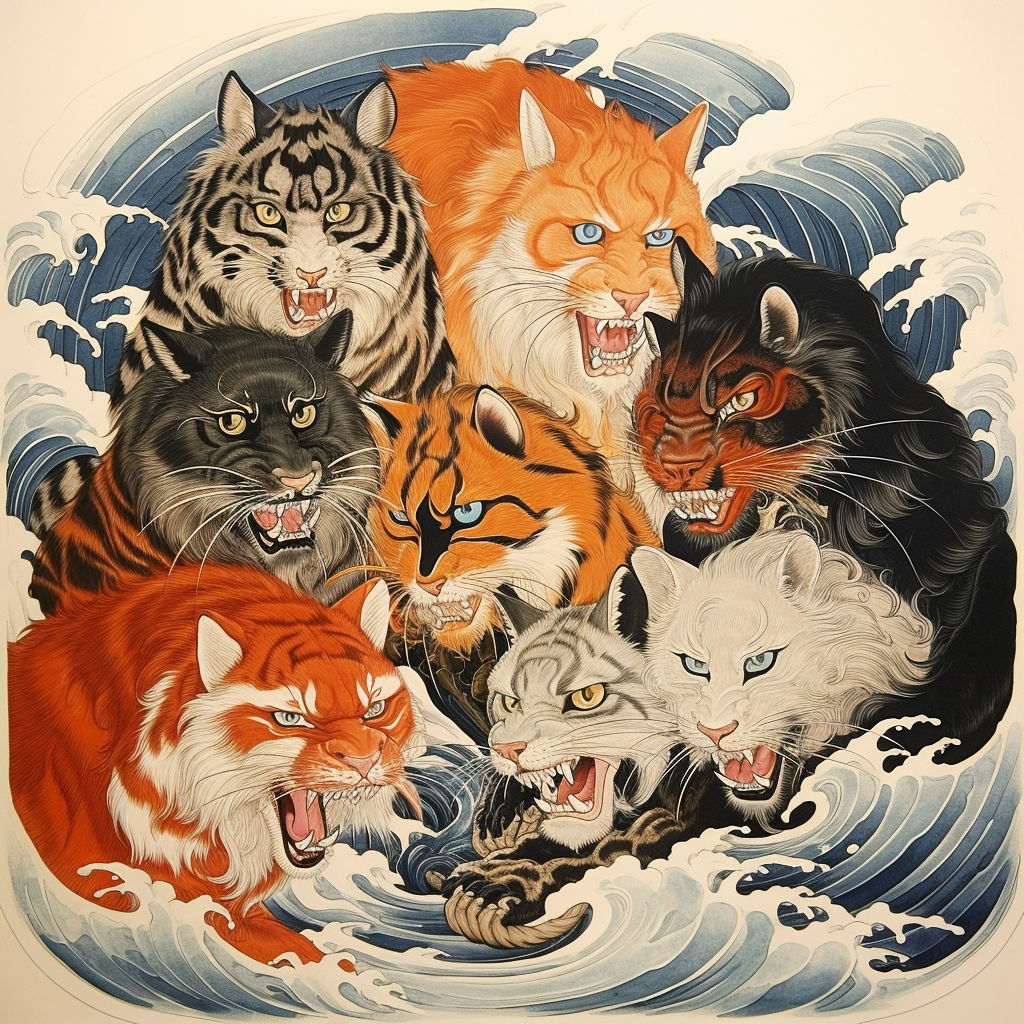
\includegraphics[height=4cm]{images/the_team}
%\end{minipage}

\end{frame}

%%------------------------%%

\begin{frame}
\frametitle{Inclusive DIKU}
\begin{minipage}{0.5\linewidth}
\begin{itemize}
\item Welcome to DIKU. Our goal is to promote excellence in computer science education and research. 
\item To strive for a respectful, inclusive, diverse environment and encourage open and critical academic discussion. 
\item We strive to create a welcoming and respectful environment.
\end{itemize}
\end{minipage}
\begin{minipage}{0.4\linewidth}
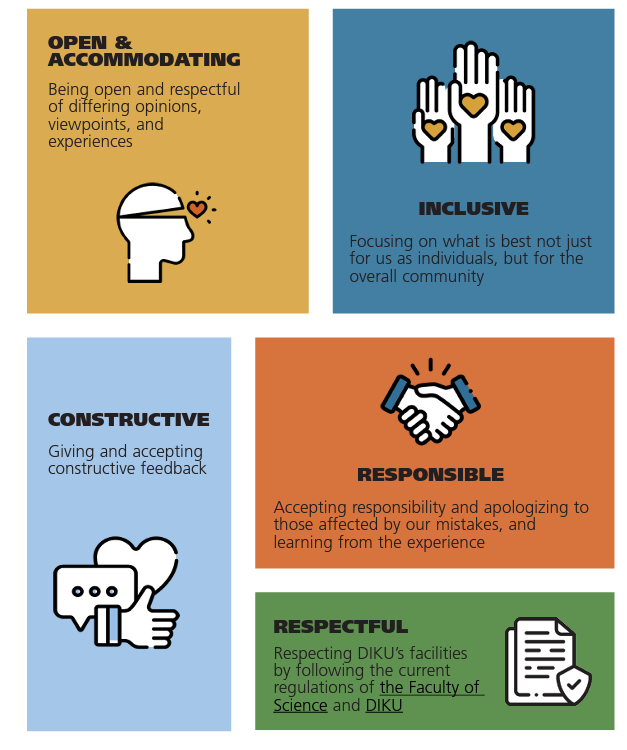
\includegraphics[height=5cm]{images/diku_cc}
\end{minipage}
\end{frame}

%%------------------------%%

 \begin{frame}
   \frametitle{Velkommen!}

   \begin{itemize}
   \item Presentation of Activities
   \item Why and what is the Kickstart course?
   \end{itemize}
 \end{frame}
 
%%------------------------%%

\begin{frame}
\frametitle{Overal Plan for the week}
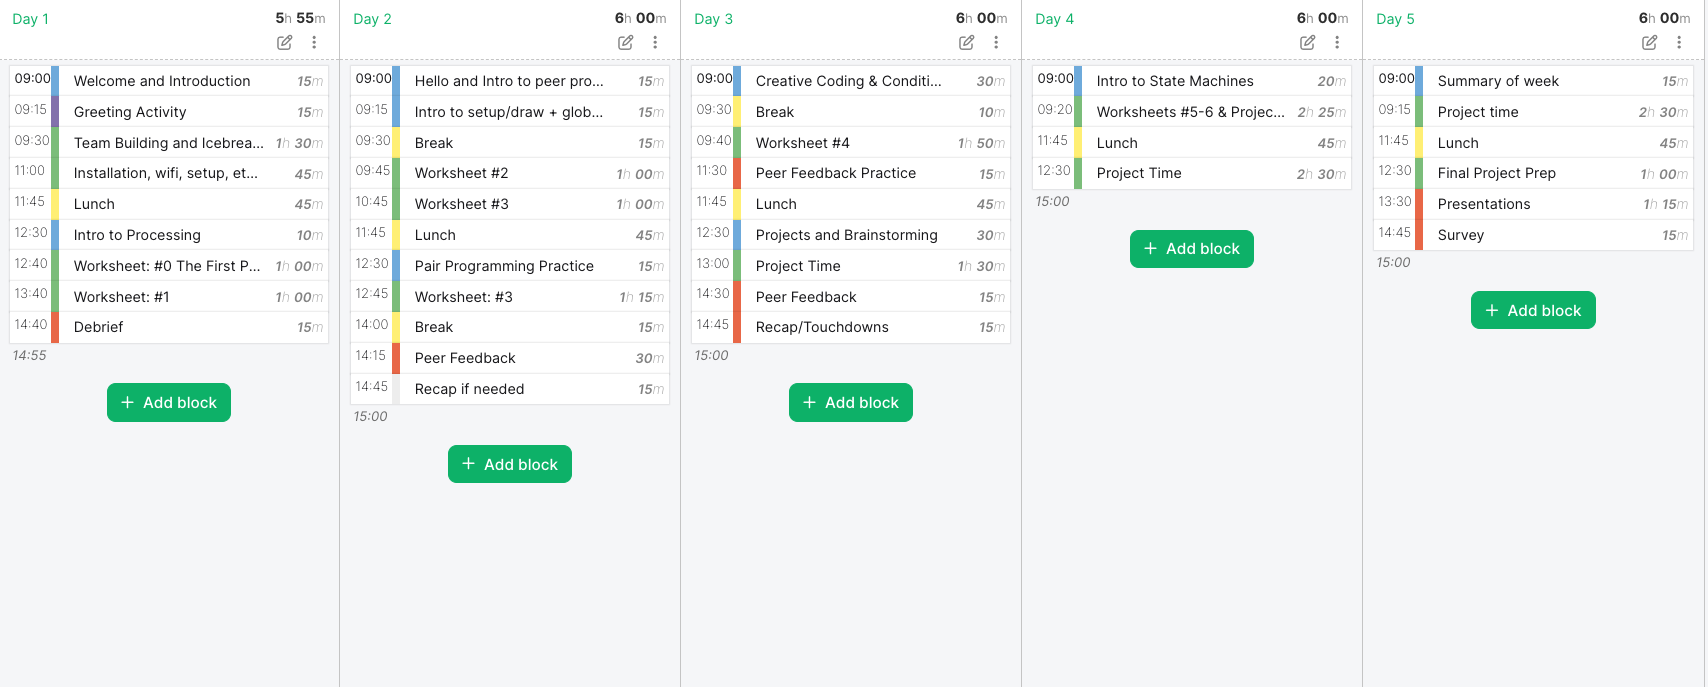
\includegraphics[height=4.5cm]{images/visual_schedule23}
\end{frame}

%%------------------------%%

\begin{frame}
  \frametitle{Monday's Plan }
  \begin{itemize}
  \item kl. 9:00-11:00 - Team Building Activities, Mini-Lecture, Code, Code, and more Code
  \item KL 11:15-11:45 - Processing Introduction
  \item kl. 11:55 - Lunch - Bio Kantine
  \item kl. 13:00-13:30 - Aud.06 Intro to Processing 
  \item kl. 13:30-14:45 - Team rooms - Intro to Processing  
  \item kl. 14:45-15:00 - Check-in with Teams
  \item kl. 15:00-? - Relax for tomorrow or code more!
  \end{itemize}
\end{frame}
 
%%------------------------%%

\begin{frame}
 \frametitle{Intended Fun Outcomes}
   \begin{outline}
   \1 {Why IFOs and not Intended Learning Outcomes}
   \2{Intended Learning Outcomes (ILOs) define what a learner will have acquired and will be able to do upon completing their courses and studies.}
      \end{outline}
\end{frame}

%%------------------------%%

\begin{frame}
 \frametitle{Intended Fun Outcomes: }
   \begin{outline}
   \1 {NDAB15009U Programmering og problemløsning (PoP)}
      \2{Knowledge on:}
  	 \3{Basic concepts within the imperative, object-oriented and functional programming paradigms: Functions and methods, variables, expressions, types, control structures, loops, block structure, classes and objects, object interaction, inheritance, recursion, polymorphism, abstraction, exceptions, pattern matching over recursive data types, etc.}
	\3{Good programming practice: Documentation in the code, design patterns, testing, incl. unit testing, handling runtime errors, etc.}
	\3{Techniques for problem-solving: Technical analysis of natural language problems, object-oriented design, modelling languages, etc.}
	\3{https://kurser.ku.dk/course/ndab15009u/}
   \end{outline}
\end{frame}

%%------------------------%%

\begin{frame}
 \frametitle{Intended Fun Outcomes}
   \begin{itemize}
    \item{Meet people and collaborate}
    \item {Explore programming with a focus on creating games}
    \item{Have fun and take chances through creativity}
    \item Take control of your education
   \end{itemize}
     \hspace{8 em}
\begin{minipage}{0.4\linewidth} 
      
\includegraphics[height=4cm]{images/happy_coders}
\end{minipage}

\end{frame}


%%------------------------%%
\section{Icebreaking}
\begin{frame}
 \frametitle{Meet people and collaborate}
 \begin{itemize}
   \item {Design Thinking}
    \item{Collaboration}
    \item{Reframing}
 \end{itemize}
\end{frame}

%%------------------------%%

\begin{frame}
 \frametitle{Teams and Instructors}
 \begin{itemize}
 \item{\textbf{Team Alpha:} Christian and Casper, room A105}
 \item{\textbf{Team Bravo:} Nanna and Nicolaj, room A106}
 \item{\textbf{Team Charlie:} Anders and Laufey, room A107}
 \item{\textbf{Team Delta:} Sofie and Jeppe, room A110}
\end{itemize}
\begin{minipage}{0.4\linewidth} 
      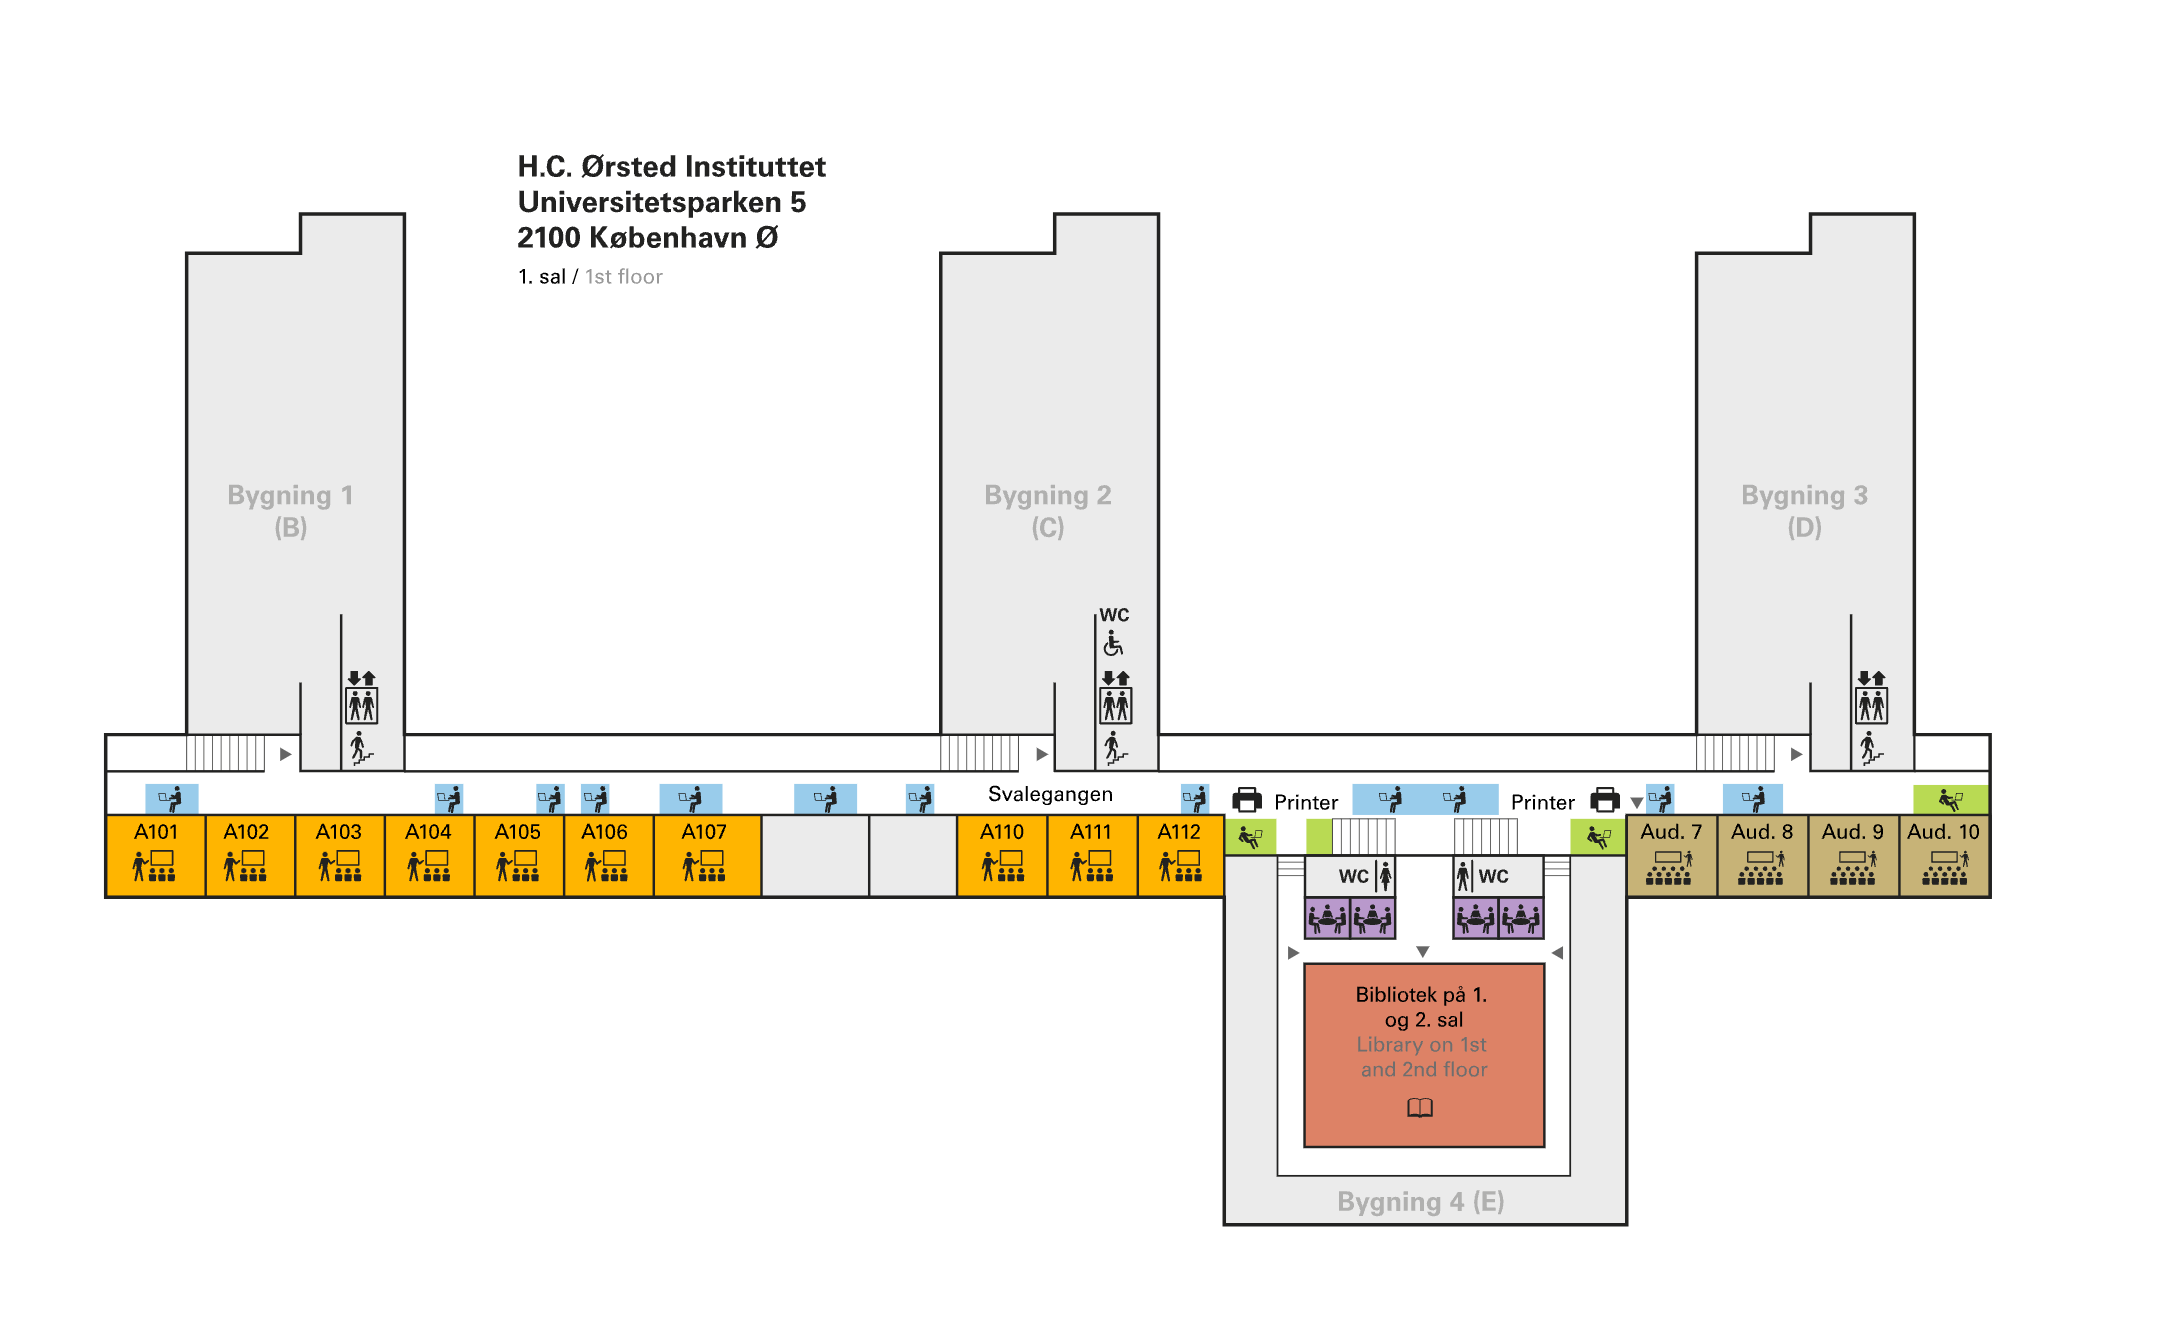
\includegraphics[height=6cm]{images/team_rooms}
\end{minipage}
\end{frame}

%%------------------------%%
\begin{frame}
 \frametitle{Challenge Time}
 \begin{itemize}
   \item {Design Thinking}
    \item{Collaboration}
    \item{Reframing}
 \end{itemize}
\end{frame}

%%------------------------%%
%% VIDEO
%%------------------------%%

\begin{frame}
 \frametitle{Time for Challenge}
   \vspace{5 mm}
    \hspace{8 mm}

  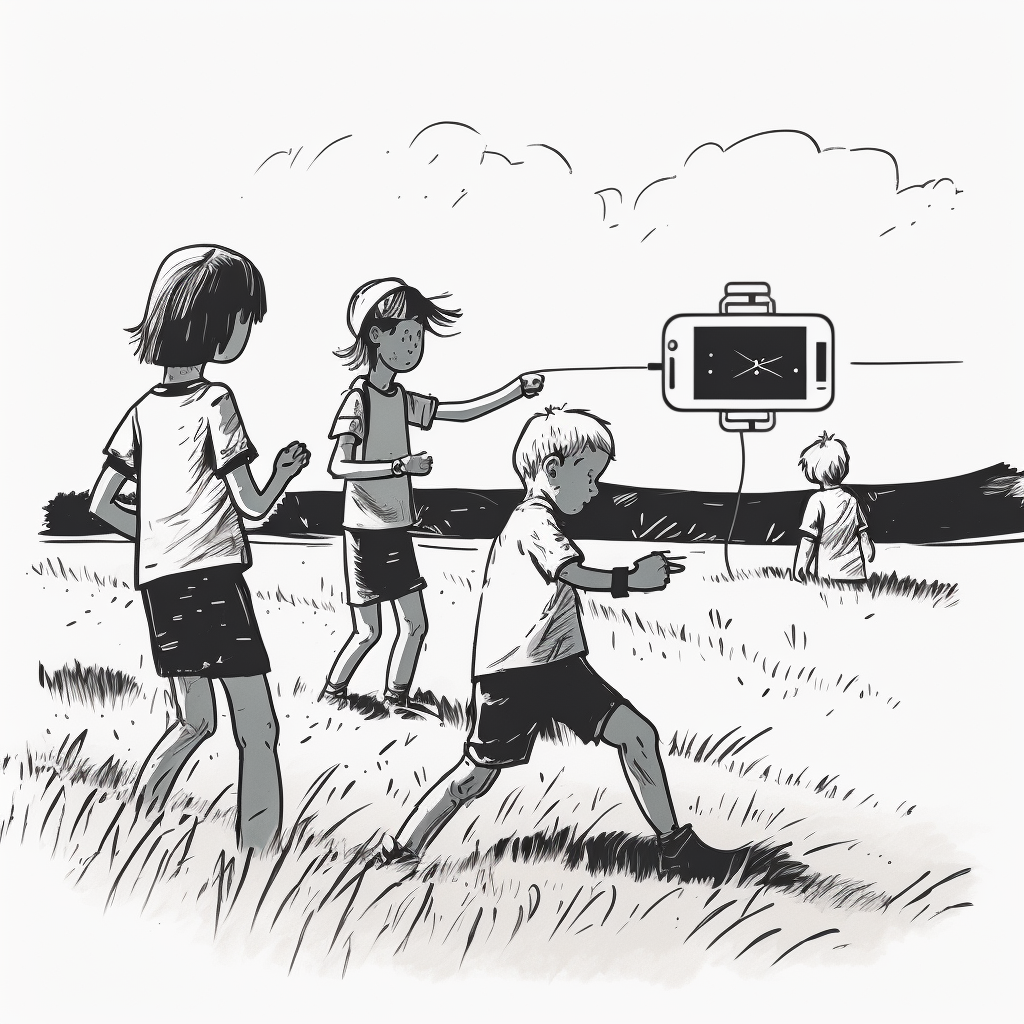
\includegraphics[height=8cm]{images/challenge_time}

\end{frame}

\begin{frame}
   \frametitle{Marshmallow Challenge Reflection}
   	\begin{itemize}
	\item {\href{https://www.ted.com/talks/tom_wujec_build_a_tower_build_a_team?utm_campaign=tedspread&utm_medium=referral&utm_source=tedcomshare}{TED TALK Tom Wujec}}

		\item{Constant prototyping as a problem-solving method.}
		\item{Getting the Design Right and the Right Design, Buxton, William (2007). Sketching user experiences: getting the design right and the right design. Amsterdam: Elsevier/Morgan Kaufmann }
			\end{itemize}
\end{frame}


%%------------------------%%
\section{WIFI ect}
\begin{frame}
  \frametitle{Internet Access}

  Aktiver KU-bruger
  \begin{itemize}
  \item Log på \texttt{http://mit.ku.dk} med NemID og find midlertidig pinkode.
  \item Gå til \texttt{http://kunet.dk} og tryk ``Første gang du logger på''.
  \item Log på med den midlertidige kode og CPR nummer uden bindestreg.
  \item Aflæs KU brugernavn (fx \texttt{abc123}) og angiv password.
  \end{itemize}

  \vspace{5mm} 
  eduroam WiFi
  \begin{itemize}
  \item Kræver KU bruger og password
  \item Log på med brugernavn: \texttt{abc123@ku.dk}
  \end{itemize}

  \vspace{5mm} 
  Alternativt: KU Guest WiFi
  \begin{itemize}
  \item Opret 24 timers konto ved at indtaste navn, mail, mobilnummer. 
  \item Modtag kode via SMS.
  \end{itemize}
  %   \begin{textblock}{5}(2,2)
% \end{textblock}
\end{frame}

%%------------------------%%
\section{Processing}
\begin{frame}
  \frametitle{I. Installation af Processing.py}

  \begin{itemize}
  \item Hent og installer Processing fra \url{http://processing.org/download/}
  \item Installer Python Mode via library manager
  \item SEE: https://bit.ly/3SXOp4r
  \end{itemize}
   
\includegraphics[height=3cm]{images/propy06}
  %   \begin{textblock}{5}(2,2)
% \end{textblock}
\end{frame}

%%------------------------%%

\begin{frame}
  \frametitle{II Installation af Processing.py}
   
   \vspace{10 mm}
    \hspace{8 em}
   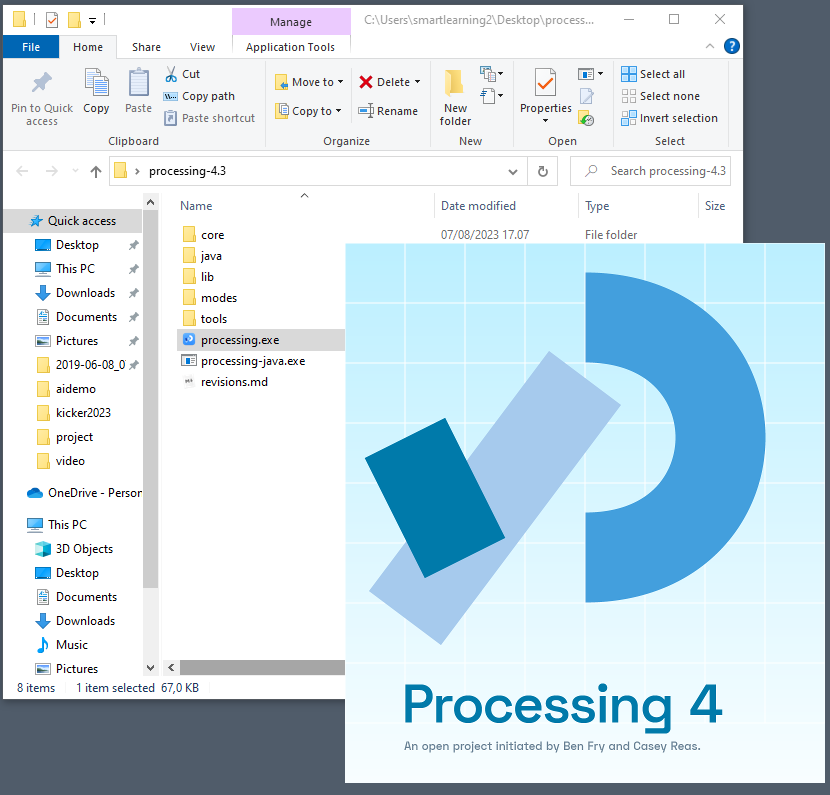
\includegraphics[height=6cm]{images/python00}
\end{frame}

\begin{frame}
  \frametitle{III. Installation af Processing.py}
   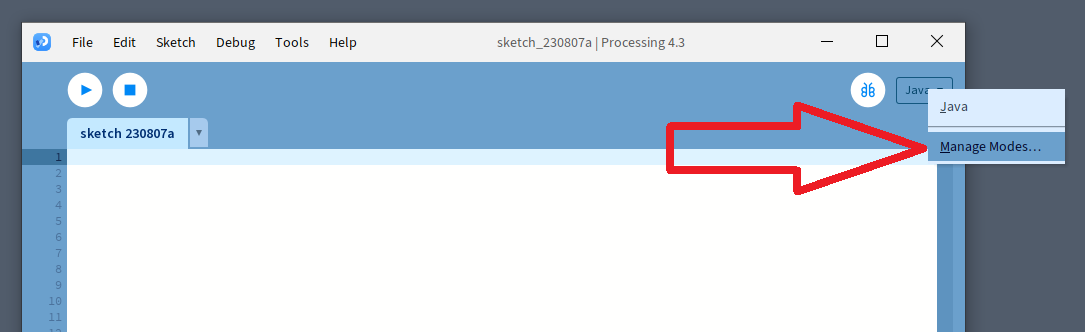
\includegraphics[height=3cm]{images/python01}
\end{frame}

\begin{frame}
  \frametitle{IV. Installation af Processing.py}
   \vspace{10 mm}
    \hspace{8 em}
   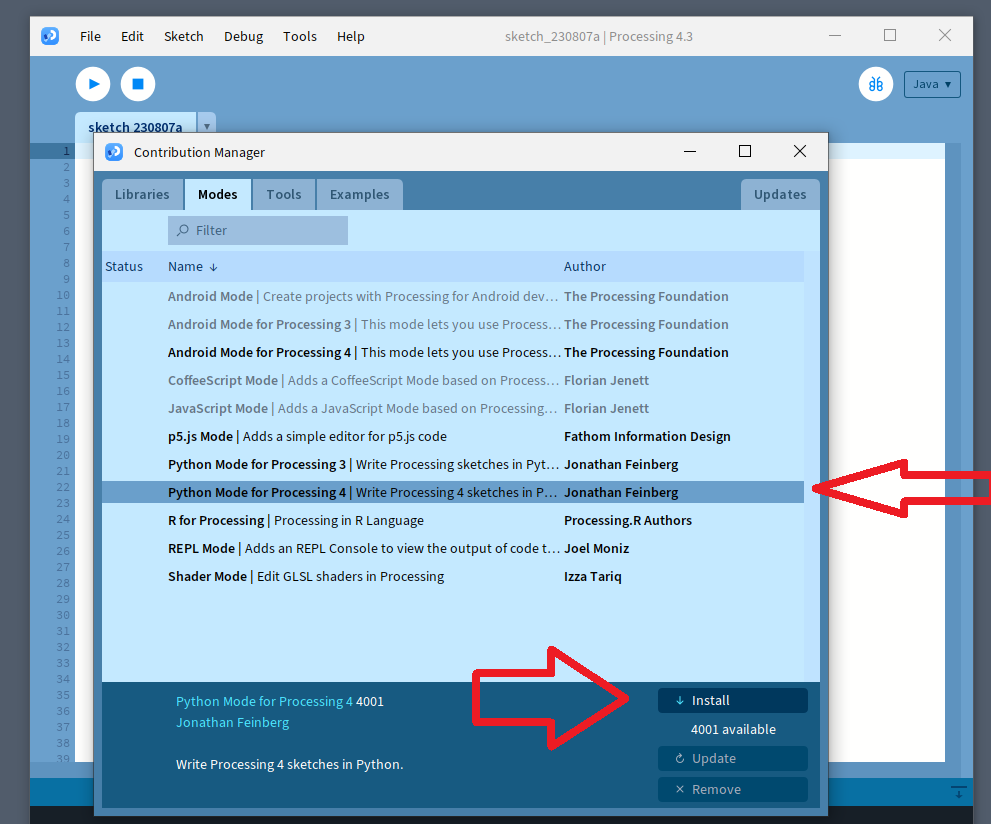
\includegraphics[height=6cm]{images/python02}
\end{frame}

%%------------------------%%

\begin{frame}
  \frametitle{V. Installation af Processing.py}
  \vspace{10 mm}
    \hspace{8 em}
   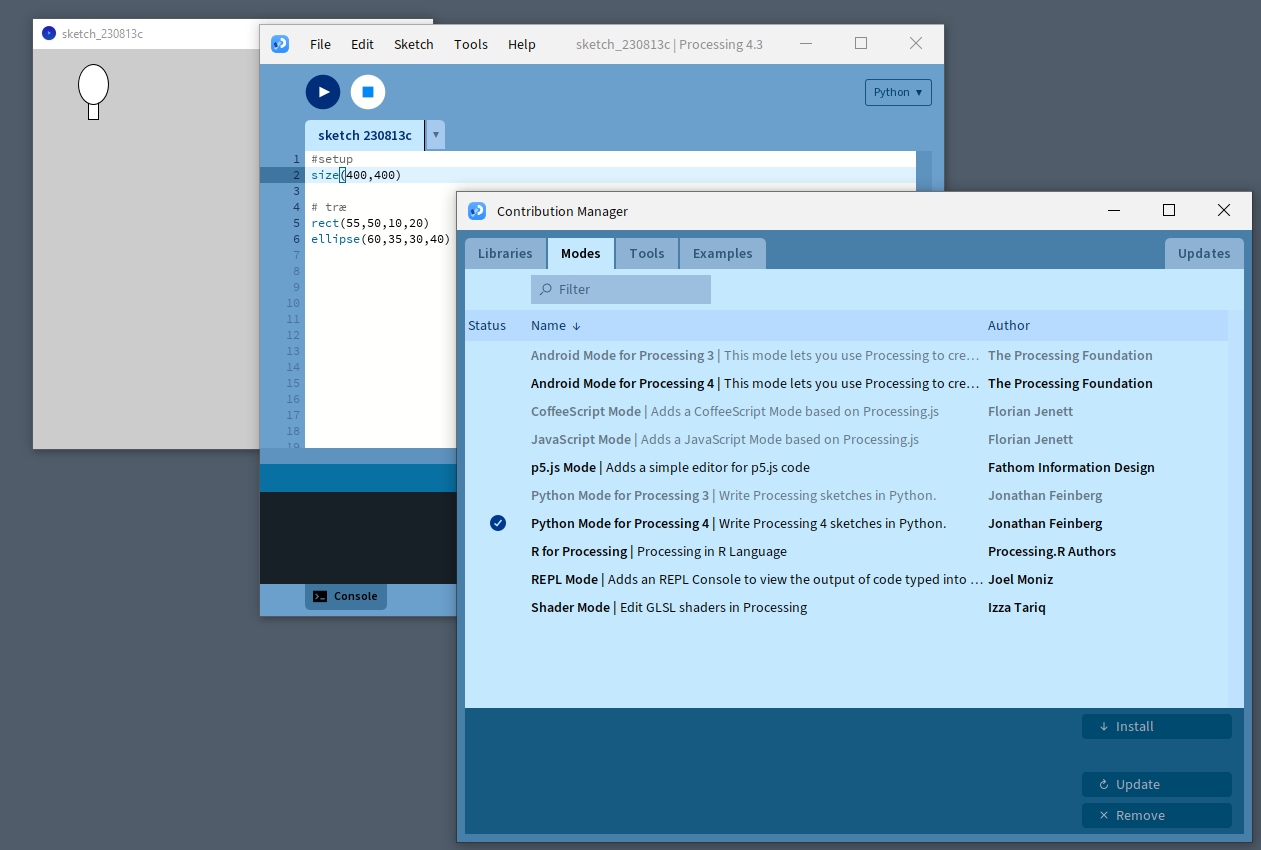
\includegraphics[height=6cm]{images/python03}
\end{frame}


%%------------------------%%
\begin{frame}
 \frametitle{Lunch}
   \vspace{5 mm}
    \hspace{8 mm}

  \includegraphics[height=7cm]{images/lunch}

\end{frame}




%%------------------------%%

%% What is Processing 5 %%

%%------------------------%%

\begin{frame}
   \frametitle{Processing History}
   	\begin{itemize}
	\item M.I.T. Media Lab Casey Reas \& Ben Fry
	\item Design By Numbers  - Maeda, John. - Design by numbers / John Maeda.. - 1999. - ISBN: 0262133547
	\item Creative Programming
	\end{itemize}
	 \hspace{8 em}
   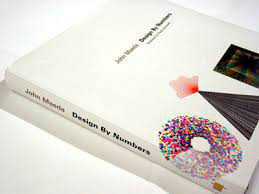
\includegraphics[height=4cm]{images/design}
\end{frame}

%%------------------------%%

\begin{frame}
   \frametitle{What is Processing}
   \begin{itemize}
   \item {Processing is a flexible software sketchbook and a language for learning code. Since 2001, Processing has promoted software literacy within the visual arts and visual literacy within technology. Thousands of students, artists, designers, researchers, and hobbyists use Processing for learning and prototyping.}
   \item{Processing Development Environment $\rightarrowtail$ PDE}
   \item{Programs are called Sketches}
   \item{The PDE consists of a simple text editor for writing code, a message area, a text console, tabs for managing files, a toolbar with buttons for common actions, and a series of menus.}
\end{itemize}	
%\hspace{8 em}
%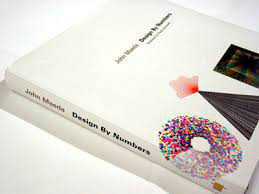
\includegraphics[height=4cm]{images/design}
\end{frame}

%%------------------------%%
\begin{frame}
  \frametitle{Processing Example}
  \vspace{3mm}
  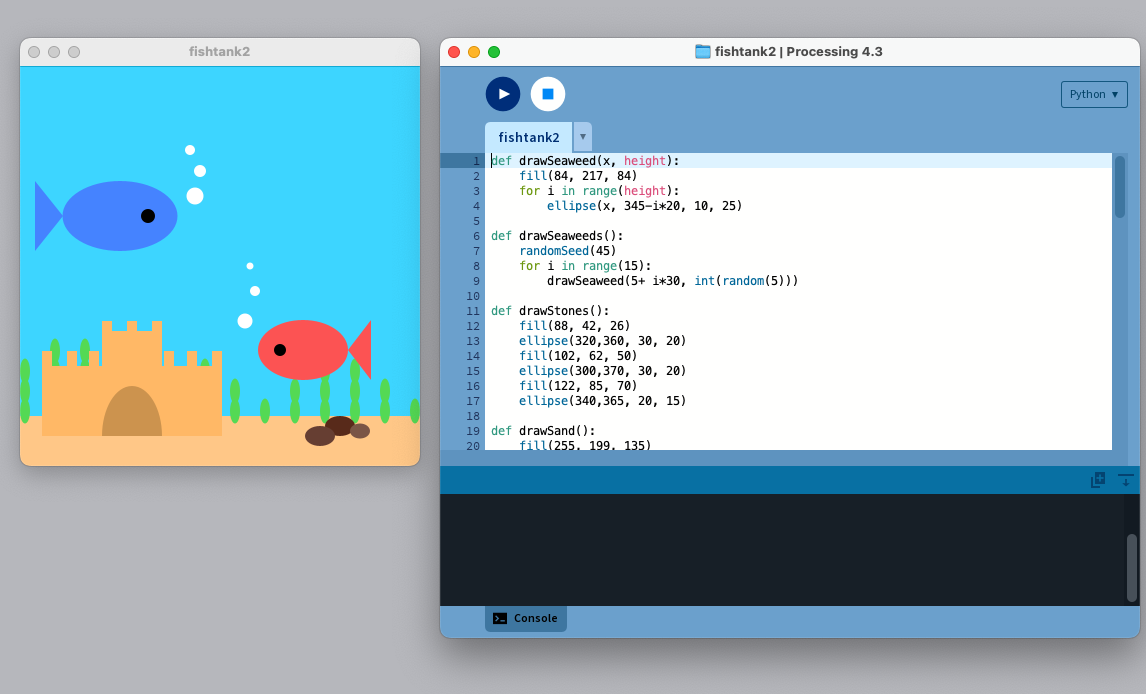
\includegraphics[width=0.8\textwidth]{images/python04}
\end{frame}

%%------------------------%%

\begin{frame}
\frametitle{Processing Parts 1}
\begin{enumerate}
\item
  \textbf{Basics of Processing IDE:}

  \begin{itemize}
  \item
    \textbf{Interface:} The Processing IDE has a simple interface.
    There's an area for writing code, buttons for running and stopping
    sketches, and a message area below for error messages and other
    notifications.
  \item
    \textbf{Sketch:} In Processing, each project is called a "sketch". A
    sketch is a combination of code, data, and output.
  \end{itemize}
\item
  \textbf{Language:} Processing uses a variant of the Java language.
  It's designed to be beginner-friendly, with simpler functions and
  setup to create visual and interactivey projects quickl.
\item
  \textbf{Structure of a Basic Sketch:}

  \begin{itemize}
  \item
    \textbf{\texttt{setup()} function:} This is executed once when the
    sketch starts. It's commonly used to define initial environment
    properties such as screen size and background color.
  \item
    \textbf{\texttt{draw()} function:} This runs repeatedly after
    \texttt{setup()}. It's used for continuously running code, such as
    animation or checking for input.
  \end{itemize}
\item
  \textbf{Running the Sketch:} The sketch is compiled and run when you
  click the "Run" button (or press Ctrl+R/Cmd+R). The visual output is
  displayed in a separate window.
\end{enumerate}
\end{frame}

%%------------------------%%

\begin{frame}
\frametitle{Processing Parts 2}
\begin{enumerate}
\item
  \textbf{Libraries and Extensions:} Processing has a range of libraries
  that can be imported to add functionality, such as handling video,
  sound, or advanced graphics operations.
\item
  \textbf{Exporting:} You can export your sketches to standalone
  Windows, macOS, and Linux applications. Exporting projects for the web
  using the P5.js variant of Processing is also possible.
\item
  \textbf{Modes and Variants:}

  \begin{itemize}
  \item
    \textbf{P5.js:} A JavaScript library with the essence of Processing
    but for web development. It brings the Processing approach to web
    artists and developers.
  \item
    \textbf{Python Mode:} Allows you to write Processing sketches in
    Python.
  \item
    \textbf{Android Mode:} This lets you create Android apps using the
    Processing API.
  \end{itemize}
\item
  \textbf{Community:} One of the strengths of Processing is its active
  and supportive community. Numerous tutorials, forums, and resources
  are available to help users learn and troubleshoot.
\end{enumerate}
\end{frame}

%%------------------------%%

\begin{frame}
\frametitle{Enough Lecture: Today's IFOs}
\begin{itemize}
\item{You will get a sense of the PDE shortly}
\item{How to \textbf{draw and color} with Processing}
\item{What are \textbf{Variables} as simple as they get}
\end{itemize}
\end{frame}

%%------------------------%%

\begin{frame}
\frametitle{Enough Lecture: Today's IFOs}
\begin{itemize}
\item{You will get a sense of the PDE shortly}
\item{How to \textbf{draw and color} with Processing}
\item{What are \textbf{Variables} as simple as they get}
\end{itemize}
\end{frame}


%%------------------------%%

\begin{frame}
  \frametitle{Drawing}
   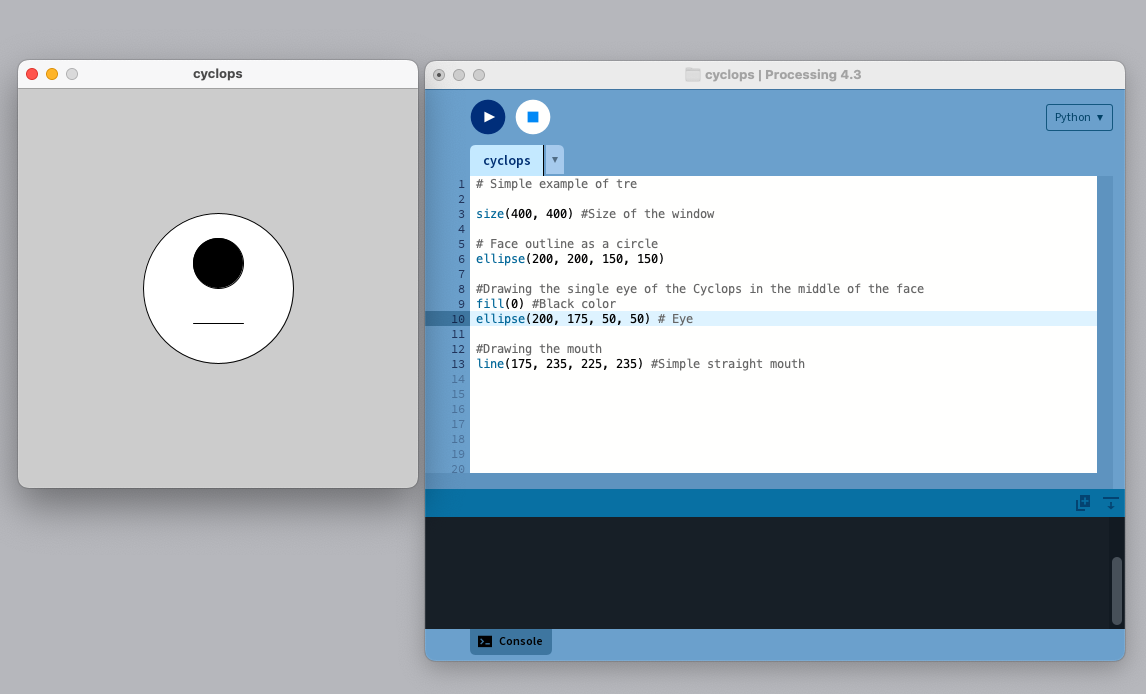
\includegraphics[width=0.9\textwidth]{images/drawing_01}
  
  \end{frame}

%%------------------------%%

\begin{frame}
  \frametitle{Variables}
  \begin{itemize}
   \item{At its core, a \textbf{variable in programming} is like a container or a storage box that holds data.}
   \item{\textbf{Variables} are names that hold \textbf{values}.}
    \item{Imagine you have a box in real life where you put an apple; you might label that box "fruit" so you know it contains a fruit. In programming, the box is the variable, the apple is the data, and the label "fruit" is the variable's name..}
      \item{Keep in mind that, unlike real life, if you put in orange into your variable, it will make the apple value disappear}
 \end{itemize}
\end{frame}

%%------------------------%%

\begin{frame}
  \frametitle{Processing References}
   \begin{itemize}
   \item  \href{https://py.processing.org/reference/}{Processing Reference}
   \item  \href{https://py.processing.org/tutorials/}{Processing Tutorials}
   \end{itemize}
    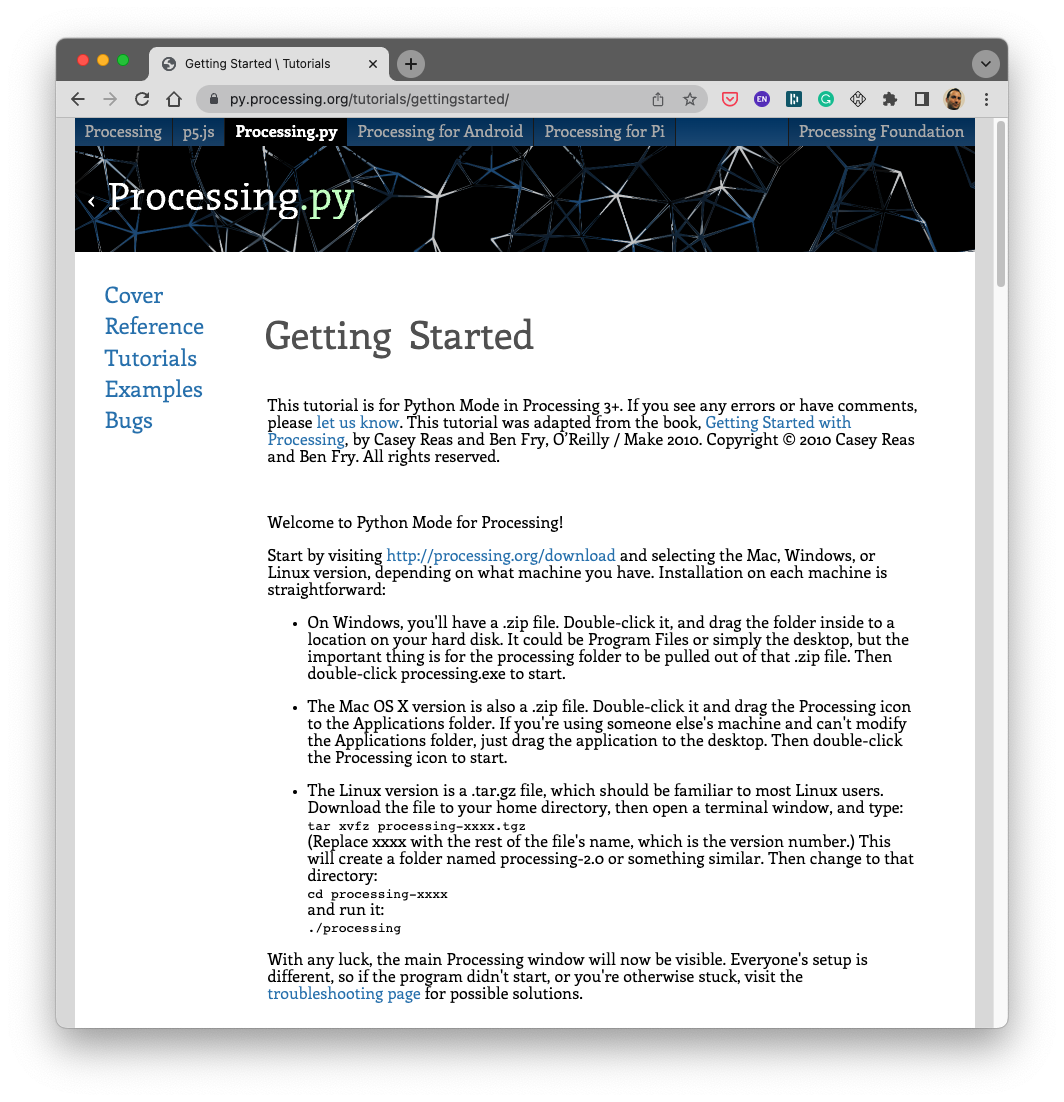
\includegraphics[width=0.6\textwidth]{images/python06}
  \end{frame}
  
%%------------------------%%

\begin{frame}
  \frametitle{Coordinate System in Processing}
   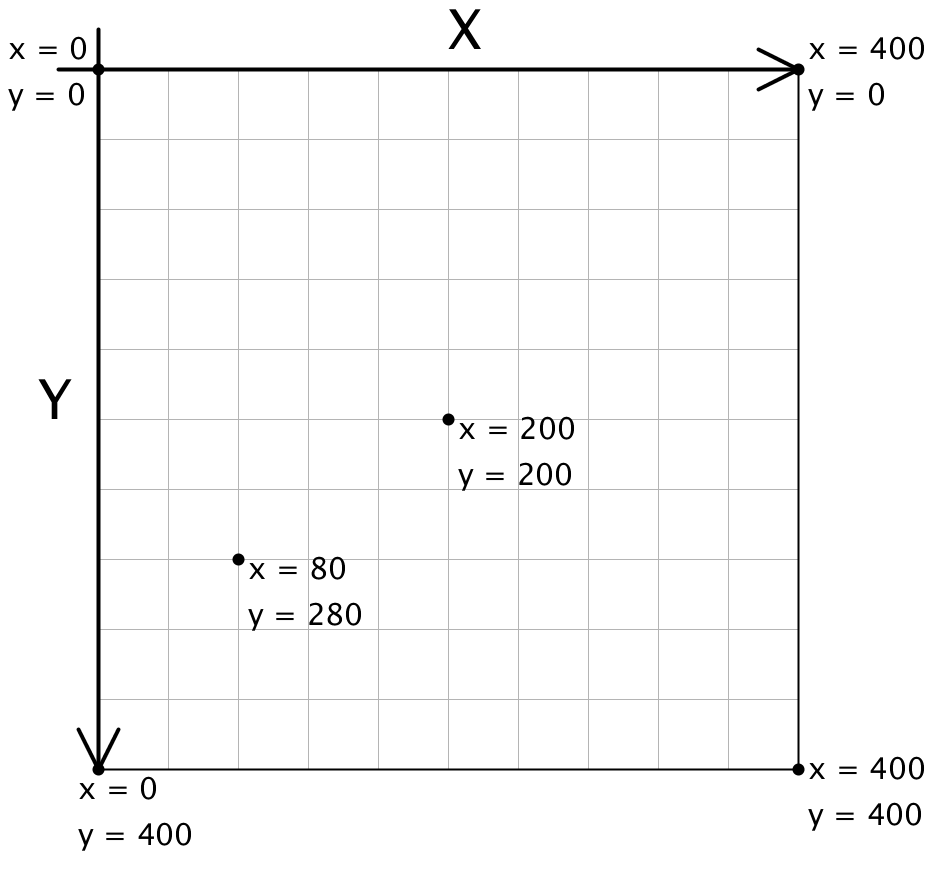
\includegraphics[width=0.8\textwidth]{images/koordinatsystem}

  \end{frame}


\end{document}